To validate the system and algorithms previously defined, several integration tests are carried out. The camera used and the additional source of light are not the same as the one described above, and they are performed on Earth, thus the verification of the system will not be complete. Nevertheless, it will be enough to, at least, confirm that the approach is achievable and needs to be further investigated. 

\section{Equipment Employed for the Experiments}
To carry out the experiments, we should build the system designed in the previous part. However, to saving time and money, it is decided to use an alternative equipment, easier to obtain, with a behavior similar to the chosen one. The components of the new system are described below.

\subsection{Lab Webcam Philips SPZ2000}
First, to carry out all the experiments, a camera to acquire the images of the scene is needed. As the camera designed in the Scene Analysis have to be built with expensive constituents, and we didn't have a lot of time, it was decided to use the webcam in the lab as a substitute. They are not accurate and their image is blurred when the object to focus is too far from it but if the algorithms compute the right distances with such a camera, a more advanced one will be capable to obtain the same or even more precise results. However, some information such as the focal length and the pixel size of the CCD are unknown. A preliminary calibration to determine the focal length and the lens distortion will be achieved before performing the experiment.

\subsection{Laser Pointer}
To simulate the additional source of light, a laser pointer is used. Only one beam is needed to perform the experiment, thus no other system will be added to split the ray. The wavelength of the laser is 532 nm, like the color chosen in the design part. Its maximum output power is 5 mW which corresponds to the order of magnitude selected before. It may not be enough to outshine the sun, but it is adequate for checking the algorithms indoor. It is powered with batteries which will not be adapted on Mars as the rover should be autonomous. 

\subsection{Computer}
On the rover, it is a micro-controller which will provide the computational power to carry out the image analysis and the calculation of the distance of the beam spots detected. As we are only testing the algorithms, and not implementing the whole system designed, a computer connected to the webcam to retrieve the images acquired is used. 

\section{Parameters of the Webcam}
As the datasheet of the webcam employed to carry out the experiments is not exhaustive, we need to establish its focal length and the impact of the lens distortion.

\subsection{Determination of the Focal Length}
Two techniques are used to find the focal length: the triangulation method and the Matlab Camera Calibration Toolbox \cite{matlabtoolbox}.

\subsubsection{Triangulation Method}
The first approach consists in placing an object whose size is known at a certain distance of the webcam and in taking a picture of it. The figure \ref{fig:schema1D} can be taken as a reference, where z is the distance camera-object, a the size of the object, p the size of the object in the image plane and $f_o$ the focal length that we want to determine. With the Thales' Theorem, it is deduced:
\begin{equation}
\frac{f_0}{z} = \frac{p}{a}
\label{eq:focal}
\end{equation}
As we measure the size of the object in the image plane in pixels, it is needed to convert it in meters. Thus, the size of each pixel of the CCD has to be known, which is not the case since the datasheet does not provide this information. However, by looking at the formula \eqref{eq:formule1D_2}, it can be noticed that we need the ratio $\frac{Pixel Size}{f_0}$ and not $f_0$ alone. This means that by deriving \eqref{eq:focal} using $p = P_{pixel} \times Pixel \ Size$ on the \textbf{x} direction, we obtain our desired ratio:
\begin{equation*}
\frac{Pixel \ Size}{f_0} = \frac{a}{Z \times P_{pixel}}
\end{equation*}

The ratio is calculated for an object of 1 m, at a distance of 5.21 m, which corresponds to 147 pixels in the image plane. It is equal to $0.0013 \ pixel^{-1}$ . This ratio is used to compute the distance object-target in the experiments but as it depends a lot of parameters measured by hand, another solution, more accurate as it is based on the cross correlation of several images is considered. 

\subsubsection{Camera Calibration}
Camera features, which include the focal length, can be obtained thanks to the Matlab Camera Calibration Toolbox \cite{matlabtoolbox}. Several pictures of a checkerboard are taken, changing the orientation of the checkerboard and its position in the image. The Matlab Single Camera Application App analyses these images and detects the intersections between four squares of the checkerboard as it can be seen in green on the figure \ref{fig:checkerboard} (Appendix \ref{Toolbox}). The origin is in yellow. Once this step achieved and the real size of one square known (39 mm here), the camera intrinsics, extrinsics and lens distortion parameters are estimated by a technique called geometric camera calibration. It uses the intersections coordinates of the checkerboard in different configurations and the factor scale to model the camera by a camera matrix which permits to transform the world coordinates into pixel coordinates on the image plan.

\paragraph*{Extrinsics Parameters}
~\\
The extrinsics parameters composed of a rotation matrix and a translation convert the world coordinated into the camera coordinates. As we are already doing this computation with our own method, these parameters are not relevant for us. Nevertheless, it can be noticed (see figure \ref{fig:extrinsics} in Appendix \ref{Toolbox}) that the Matlab functions locate accurately the position of the checkerboard. The Z coordinate is found to be around 1 m 40 and that is at that distance that the experiment was performed. Their angle seen by the camera is also precise. The correlation between several images is proved to be efficient to find the distance of a geometric image but it is not feasible on Mars soil.

\paragraph*{Intrinsics Parameters}
~\\
The intrinsics parameters are composed of the focal length and of the coordinates of the optical center in the image plan (see Table \ref{intrisicsPara}). The focal length is given in pixels in the X and Y directions. 

\begin{table}[H]
\centering
\caption{Intrinsics Parameters with Estimation Errors}
\label{intrisicsPara}
\renewcommand{\arraystretch}{1.5}
\begin{tabular}{|c|c|c|}
\hline
Intrinsic Parameters & Focal Length (in pixels) & Optical Center (in pixels)\\ \hline
Direction x & 826 $\pm$ 33 & 378 $\pm$ 29 \\ \hline
Direction y &  805 $\pm$ 31 & 175 $\pm$ 34 \\ 
\hline
\end{tabular}
\end{table}

As $f_x = \frac{f_0}{Pixel \ Size_{\text{x}}}$, we can compare the ratio previously calculated thanks to measurements to the $f_x$ found by calibrating the camera with the Matlab Toolbox. Taking into account the errors:
\begin{equation*}
Ratio = \frac{1}{f_x} \in \ [0.00116 \quad 0.00126] \ pixel^{-1}
\end{equation*}

Taking the mean of this fraction, the error between the two ratios is of 7 \%. As even the ratio with the Matlab Toolbox is not accurate since the lower bound is increased by 8.7 \% to get the upper bound, it is decided to use this calibration ratio for 1 beam spot integration testing only. Regarding the experiment with a row of points, as it was carried out for the same distance as the focal length computed by the triangulation method, the first ratio is kept. 

\subsection{Discussion About the Lens Distortion}
The smaller the lens is, the more is the chance that lens distortion occurs. The Toolbox allows us to consider the radial and tangential distortions. According the the documentation \cite{matlabtoolbox}, the latter "occurs when the lens and the image plane are not parallel" and the first one "when light rays bend more near the edges of a lens than they do at its optical center". To account for the lens distortion in our model, which could permit to obtain more accurate results as the webcam could not be perfect, the two distortions are applied to the distance in pixel between the center of the image and the optical center (computed by Matlab, see Table \ref{intrisicsPara}) and between the the centroid studied and the optical center. The difference between the two distances distorted gives us the distorted distance between the center of the image and the centroid, used to calculate the depth map. The formula to find the distortion  in the \textbf{x} direction can be found below:
\begin{equation}
\text{x}_{distorted} = \text{x}(1 + k_1 \cdot r^2 + k_2 \cdot r^4) + 2p_1 \cdot x \cdot y + p_2(r^2 + 2\text{x}^2)
\end{equation}
Where $\text{x}$ and y are the undistorted distance to the optical center, normalized by the focal length in pixel, $r^2 = \text{x}^2 + y^2$, $k_1$ and $k_2$ the radial distortion coefficients and $p_1$ and $p_2$, the tangential ones given by the Calibration App.

\section{Determination of the Depth of One Laser Beam}
In this first integration test, we would like to establish the distance from the camera to one specific point of a surface, before checking the algorithms for several points. The general procedure is detailed below. 

\subsection{General Procedure}
As the angle between the focal axis of the camera and the focal axis of the light source is easier to obtain when the laser and the camera are aligned, they need to be located on the same axis for the experiment (see figure \ref{fig:experiment1point}). Once they are placed, the distance \textbf{d} between them is measured. Then a surface is required to project the laser beam. As it is more convenient to have a mobile surface to be able to move easily the target, we choose to use a blackboard for the test (figure \ref{fig:blackboard}). The green is dark enough to contrast with the light green spot and the albedo of this surface is not very important which illustrates one of the worst case of the reflective power of a martian rock. The distance from the blackboard to the camera is measured to calibrate the system.

\begin{figure}[!h] 
\centering
\subfigure[System Camera-Laser]{
  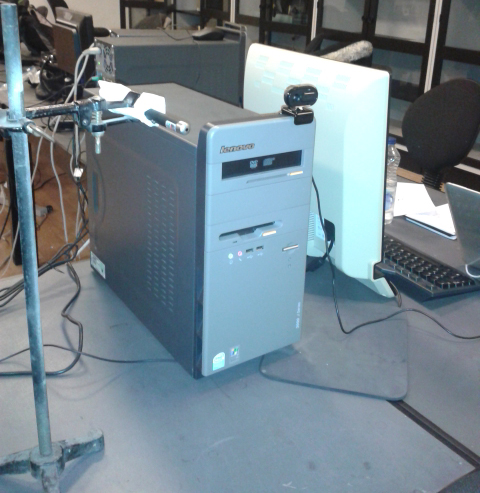
\includegraphics[scale=0.35]{fig/CamLaser.jpg}
  \label{fig:experiment1point}
}
\quad 
\subfigure[Blackboard]{
  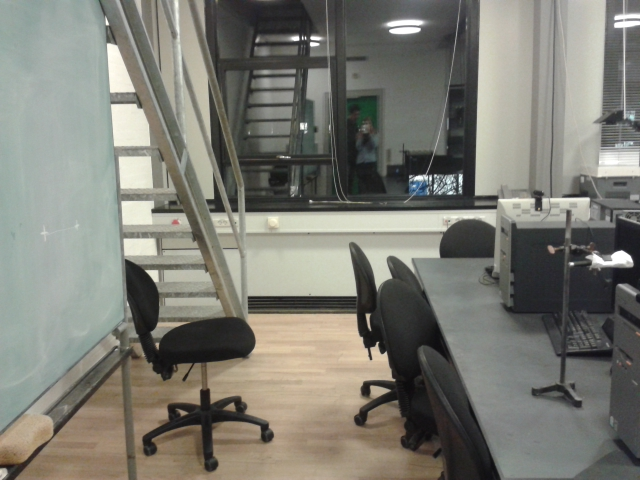
\includegraphics[scale=0.35]{fig/BlackBoard.jpg}
  \label{fig:blackboard}
}
\caption{System Camera-Laser-Blackboard} 
\end{figure}

\subsubsection{Calibration}
Two calibrations need to be accomplished before carrying out the 3D map of the point: setting the laser position and tuning the parameters thanks to the trackbars to detect the point.
\paragraph*{Material}
~\\
The webcam is connected to the computer and the calibration program is run. It only consists in acquiring frames from the webcam and displaying them on the screen of the computer. A cross is added in the center of each image to facilitate the calibration. The purpose of this step is to obtain the spot projected by the laser at the center of the image. Indeed, once this achieved, we get easily the angle $\alpha$ between the focal axis of the camera and the one of the light source, needed to compute the depth map. It can be deduced from the figure \ref{fig:schema1D} that $tan(\alpha) = \frac{d}{z}$, where d is the distance camera-laser and z the distance camera-blackboard.

\paragraph*{Color Detection}
~\\
Once the laser position is set, the color detection program is started. The parameters need to be tuned to detect the bright green color of the beam spot. As we are dealing with only one point, it is not imperative to add erosion or dilation to make an opening. The noise can be discarded with only the expected pixel size of the spot in the image plane. Thus, only the HSV values are changed to match the green of the point.

\subsubsection{Distance Computation}
The calibration accomplished, the distance can be calculated either in real time since frames for the webcam are acquired quickly and the processing is short, either later on, using pictures saved after the calibration steps at different positions of the blackboard.

\subsection{Experiment and Results}
The general procedure described is implemented with the distance camera-laser equals to 30 cm, the distance camera-blackboard equals to 137 cm, hence an angle $\alpha$ of 12.75~$\degree$. The experiment was carried out in real time and repeated a second time, handling only pictures and taking into account the lens distortion. This is the latter result which are given below in the Table \ref{results1Point}. They correspond to the image processing displayed on figures \ref{fig:exp1Point137} and \ref{fig:exp1Point98dot5}.

\begin{figure}[!h] 
\centering
\subfigure[Original Image (137 cm)]{
  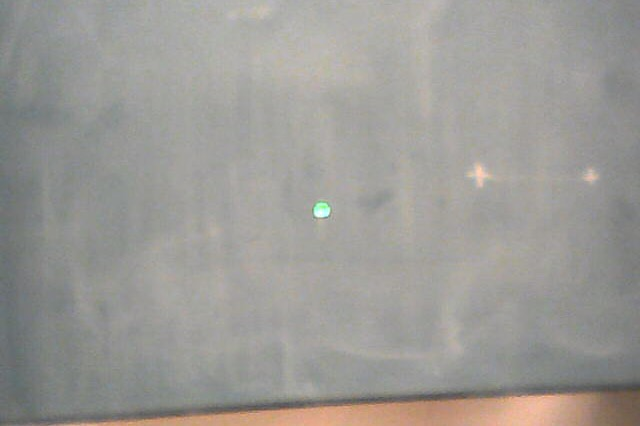
\includegraphics[scale=0.3]{fig/137cm.jpg}
  \label{fig:exp1Point137}
}
\quad 
\subfigure[HSV Image of the Point Detected (137 cm)]{
  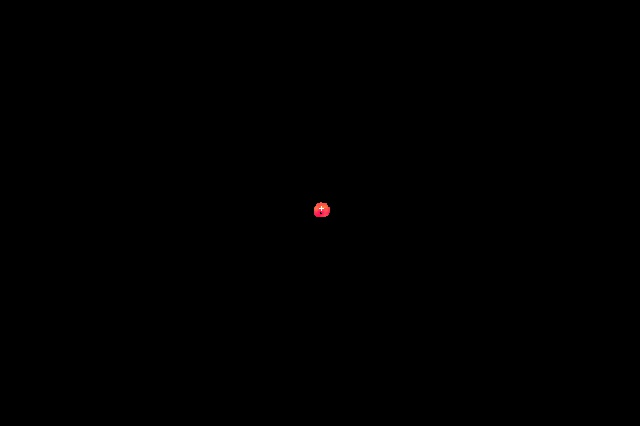
\includegraphics[scale=0.3]{fig/137PointHSV.jpg}
  \label{fig:exp1Point137HSV}
}
\subfigure[Original Image (98.5 cm)]{
  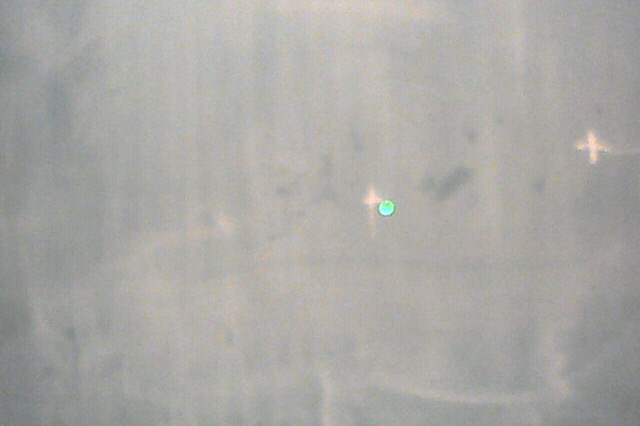
\includegraphics[scale=0.3]{fig/98dot5cm.jpg}
  \label{fig:exp1Point98dot5}
}
\quad 
\subfigure[HSV Image of the Point Detected (98.5 cm)]{
  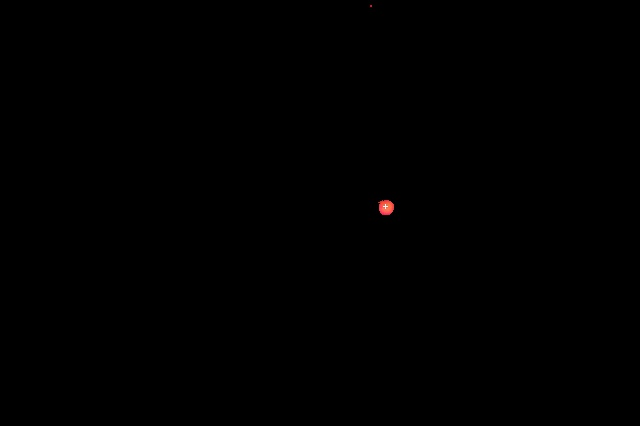
\includegraphics[scale=0.3]{fig/98dot5PointHSV.jpg}
  \label{fig:exp1Point98dot5HSV}
}
\caption{Experiment Images Acquired by the Camera and Processed for 137 cm and 98.5 cm} 
\end{figure}

\begin{table}[h]
\centering
\caption{Results of the depth mapping for 1 point with and without lens distortion}
\label{results1Point}
\renewcommand{\arraystretch}{1.5}
\begin{tabular}{|c|c|c|}
\hline
\multicolumn{3}{|c|}{Distance (cm)} \\ \hline
Camera-Blackboard & Computed without distortion & Computed with distortion \\ \hline
137 & 136.2463 & 136.2557 \\ \hline
124 & 125.2243 & 125.2153 \\ \hline
111.5 & 113.2045 & 113.1927 \\ \hline
98.5 & 100.7686 & 106.4445 \\ \hline
\end{tabular}
\end{table}

Finally, the errors with and without lens distortion are detailed in the chart \ref{chart1Point}. It can be noticed that the more the blackboard is brought closer to the camera and is moved away from its calibration position, the more the error increases. Indeed, when the blackboard is closer to the camera, the displacement of the point from the center of the image is larger (see figures \ref{fig:exp1Point137HSV} and \ref{fig:exp1Point98dot5HSV}) and the error gets bigger with the distance centroid-center of the image. Without the distortion, the inaccuracy is between 7.5 mm for 137 cm and 22.7 mm for 98.5 cm. For the latter, it is quite a large error since the rock could be nearly flat and in order to stabilize the arm, a precise 3D map needs to be carried out. If the rock relief is in the range of the millimeter, it is likely that all the results of the distances will not do any difference between several points and the stabilization could not be achieved since no specific spot could be tracked in two images acquired at different times. The errors could be caused firstly by the fact that the experimental conditions were not ideal. The distances were measured thanks to a measuring tape but the precision was only around the millimiters, and as it was not perfectly straight between the camera and the blackboard, measurement errors could occur. Moreover, the blackboard was moved several times and could have not been perfectly perpendicular to the camera optical axis. Then, the camera images were blurred and it was not designed for this kind of processing, which biased the centroiding. Also, when the point is detected, it could have less or more pixels than the original point, used for the calibration. That means that the center of mass could be displaced and create important errors. An analysis of this error will be carried out further in the report.

\begin{figure}[!h] 
\centering
  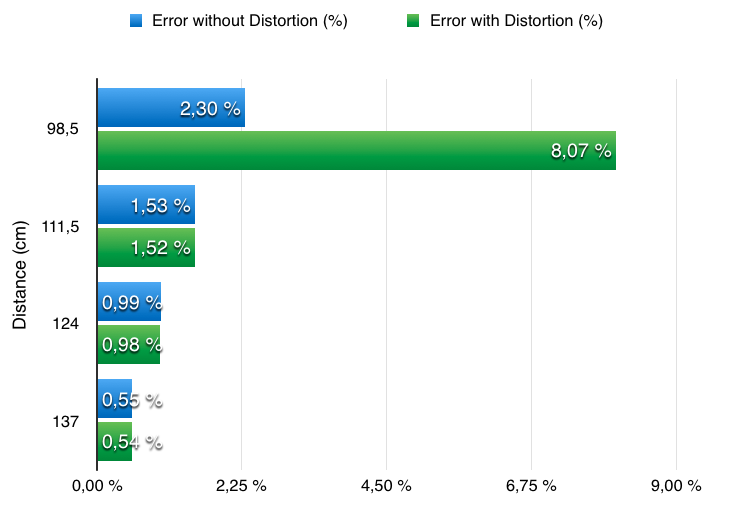
\includegraphics[scale=0.5]{fig/chart1Point.png}
\caption{Distance Errors with and without Lens Distortion} 
\label{chart1Point}
\end{figure}

Finally, the lens distortion have to be taken into account for explaining the results. Indeed, it can be observed that the error between the real distance and the computed one comes from the fact that the lens have distortions and that the distance measured between the centroid and the center of the image is inexact. To deal with this issue, the radial and tangential distortions parameters calculated by the Matlab Calibration Toolbox were added to the algorithm in order to compute the distance considering the case with the lens distortion. The results are also detailed in the Table \ref{results1Point} and the chart \ref{chart1Point}. As expected, when the distance is computed with the distance centroid-center of the image distorted, the measurement error is slightly smaller than in the case without distortion and it can be deduced that the lens distortion does not affect a lot the depth mapping. However, for the last distance, the error with distortion is not at all expected and shows either the limit of the lens distortion or that the distortion was wrongly implemented. Indeed, Matlab has estimated it for 137 cm. At this point, there were already estimation errors. As we get closer, the distorted distance increases and the errors are added. We should try to calibrate the camera at this distance or even closer and check the distortion parameters. Nevertheless, even if the error is accumulated, we should not obtain such a difference for the last distance tested. The implementation should be revised. An other solution will be to carry out this integration test with the designed camera, which should have a negligible lens distortion and be more accurate. The results should improve and the error may be tolerable.

Even if the results are not accurate and insufficient, it is a good beginning of distance approximations and with a better material and experimental conditions, they could be improved. It should also be noticed that the time of computation is low and sufficient for real time applications. Indeed, without taking into account the lens distortion, the distance is calculated in around 35 ms and when the distorted distance is also computed, the algorithms are 1 ms slower. It is now desired to find the depth of multiple points at the same time.